\documentclass[a4paper]{article}
\usepackage{geometry}
\usepackage{graphicx}
\usepackage{natbib}
\usepackage{amsmath}
\usepackage{amssymb}
\usepackage{bbm}
\usepackage{amsthm}
\usepackage{paralist}
\usepackage{epstopdf}
\usepackage{tabularx}
\usepackage{longtable}
\usepackage{multirow}
\usepackage{multicol}
\usepackage[hidelinks]{hyperref}
\usepackage{fancyvrb}
\usepackage{algorithm}
\usepackage{algorithmic}
\usepackage{float}
\usepackage{paralist}
\usepackage[svgname]{xcolor}
\usepackage{enumerate}
\usepackage{array}
\usepackage{times}
\usepackage{url}
\usepackage{fancyhdr}
\usepackage{comment}
\usepackage{environ}
\usepackage{times}
\usepackage{textcomp}
\usepackage{caption}
\usepackage{tikz}
\usepackage{multirow}


\urlstyle{rm}

\setlength\parindent{0pt} % Removes all indentation from paragraphs
\theoremstyle{definition}
\newtheorem{definition}{Definition}[]
\newtheorem{conjecture}{Conjecture}[]
\newtheorem{example}{Example}[]
\newtheorem{theorem}{Theorem}[]
\newtheorem{lemma}{Lemma}
\newtheorem{proposition}{Proposition}
\newtheorem{corollary}{Corollary}


\floatname{algorithm}{Procedure}
\renewcommand{\algorithmicrequire}{\textbf{Input:}}
\renewcommand{\algorithmicensure}{\textbf{Output:}}
\newcommand{\abs}[1]{\lvert#1\rvert}
\newcommand{\norm}[1]{\lVert#1\rVert}
\newcommand{\RR}{\mathbb{R}}
\newcommand{\CC}{\mathbb{C}}
\newcommand{\Nat}{\mathbb{N}}
\newcommand{\br}[1]{\{#1\}}
\DeclareMathOperator*{\argmin}{arg\,min}
\DeclareMathOperator*{\argmax}{arg\,max}
\renewcommand{\qedsymbol}{$\blacksquare$}

\definecolor{dkgreen}{rgb}{0,0.6,0}
\definecolor{gray}{rgb}{0.5,0.5,0.5}
\definecolor{mauve}{rgb}{0.58,0,0.82}

\newcommand{\Var}{\mathrm{Var}}
\newcommand{\Cov}{\mathrm{Cov}}

\newcommand{\vc}[1]{\boldsymbol{#1}}
\newcommand{\xv}{\vc{x}}
\newcommand{\Sigmav}{\vc{\Sigma}}
\newcommand{\alphav}{\vc{\alpha}}
\newcommand{\muv}{\vc{\mu}}

\newcommand{\red}[1]{\textcolor{red}{#1}}

\def\x{\mathbf x}
\def\y{\mathbf y}
\def\w{\mathbf w}
\def\v{\mathbf v}
\def\E{\mathbb E}
\def\V{\mathbb V}
\def\Pp{\mathbb P}
\def\one{\mathbbm{1}}

% TO SHOW SOLUTIONS, include following (else comment out):
\newenvironment{soln}{
	\leavevmode\color{blue}\ignorespaces
}{}


\hypersetup{
	%    colorlinks,
	linkcolor={red!50!black},
	citecolor={blue!50!black},
	urlcolor={blue!80!black}
}

\geometry{
	top=1in,            % <-- you want to adjust this
	inner=1in,
	outer=1in,
	bottom=1in,
	headheight=3em,       % <-- and this
	headsep=2em,          % <-- and this
	footskip=3em,
}


\pagestyle{fancyplain}
\lhead{\fancyplain{}{Homework 3}}
\rhead{\fancyplain{}{CS 760 Machine Learning}}
\cfoot{\thepage}

\title{\textsc{Homework 4}} % Title

%%% NOTE:  Replace 'NAME HERE' etc., and delete any "\red{}" wrappers (so it won't show up as red)

\author{
	Daniel Szabo \\
	9074762189\\
} 

\date{}

\begin{document}
	
	\maketitle 
	
	\begin{enumerate}
		\item \begin{enumerate}
			\item 
			The $ 0$-$1 $ loss is 
		\begin{align*}
			\E[\one [\hat x \neq x]] = \mathbb{P}(\hat x \neq x) = 1-\mathbb{P}(\hat x=x) = 1-\theta_x
		\end{align*}
	
		\item The $ 0$-$1 $ loss in this case is 
		\begin{align*}
			\E[\one[\hat x \neq x]] &= \mathbb{P}(\hat x \neq x) = 1-\sum_{k} \Pp(\hat x=x, x=k)\\
			&= 1-\sum_{k} \Pp(\hat x=x)\Pp(x=k) = 1-\sum_{k} \Pp(\hat x=k)^2\\
			&= 1- \sum_{k} \theta_k^2 = 1 - \| \boldsymbol{\theta} \|_2^2
		\end{align*}
		\end{enumerate}
	
	\item Under this, we want to minimize
	\begin{align*}
		\E[c_{x\hat x}] &= \sum_{i}\sum_{j} c_{ij}\Pp(\hat x = i) \Pp(x = j) = \sum_{i}\sum_{j} c_{i j} \theta_i \Pp(\hat x = j) = \sum_{j} \Pp(\hat x = j) \sum_{i} c_{i j} \theta_i
	\end{align*}
	Let $ C $ be the loss matrix with entries $ c_{ij} $, and $ \boldsymbol{\hat \theta} $ the parameter estimator. Then
	\[ \E[c_{x\hat x}] = \boldsymbol{\hat \theta}^T C \boldsymbol{\theta}, \]
	so the $ \boldsymbol{\hat \theta} $ that minimizes this is just $ C \boldsymbol{\theta} $.
	
	\item \begin{enumerate}
		\item Let the distribution of $ y $ have pdf $ \rho $.
		\begin{align*}
			\E[(x_t - y_t)^2] &= \int_{0}^{1} \int_{0}^{1} (x-y)^2 \rho(x) \rho(y)dx dy\\
			&= \int_{0}^{1} \int_{0}^{1} ((x-\mu)-(y-\mu))^2 \rho(x) \rho(y)dx dy\\
			&= \int_{0}^{1} (x-\mu)^2 \rho(x) dx + 2\int_{0}^{1} \int_{0}^{1} (x-\mu)(y-\mu) \rho(x) \rho(y)dx dy + \int_{0}^{1} (y-\mu)^2 \rho(y) dy\\
			&= \sigma^2 + \int_{0}^{1} (x-\mu)\rho(x) \int_{0}^{1} (y-\mu)\rho(y) dy + \int_{0}^{1} (x-\mu)^2 \rho(x) dx\\
			&= \sigma^2 + \int_{0}^{1} (x-\mu)^2 \rho(x) dx
		\end{align*}
	This is minimized at $ x_t=\mu $ deterministically, as it is strictly greater than zero and achieves zero at $ x_t=\mu $. Thus the optimal payment for $ T $ rounds is just $ T\sigma^2 $.
	\item There are many possible such measurements. We could measure according to the sample variance at time $ t $, $ \hat \sigma_t^2 = \frac{1}{t-1}\sum_{i=1}^t (y_t-\hat{\mu}_t)^2 $, where $ \hat \mu_t = \frac{1}{t}\sum_{i=1}^t y_t $ is the sample mean. The quantity to compare to would then be $ T\hat{\sigma}_t^2 $.
	\end{enumerate}
	
	
	\item 
	\begin{enumerate}
		\item Each language only has 10 samples in this case, so the prior probabilities are just each $ 1/3 $. The formula would be the same as what's given, namely
		\[ \hat p_\alpha(y= c_k) = \dfrac{\sum_{i=1}^{30} \one[y^{(i)}=c_k] + 1/2}{30 + 3/2} = \dfrac{10 + 1/2}{30 + 3/2} = \dfrac{1}{3}. \]
		I believe a more appropriate prior for this problem would be to sum over the number of characters in each language, but by the definitions given this is our prior.
		
		\item The class conditional parametersare given by the formula in the problem, namely
		\[ \hat p_\alpha(c_s | y=e) = \dfrac{\sum_{i=1}^{30} \sum_{j=1}^{M_i} \one[x_j^{(i)} = c_s, y^{(i)}=e] + 1/2}{\sum_{s'\in S}\sum_{i=1}^{30}\sum_{j=1}^{M_i} \one[x_j^{(i)} = c_{s'}, y^{(i)}=e] + 27/2}.\]
		The outputs for $ \theta_e,\theta_j,$ and $\theta_s $ are \\
		$ \theta_e $ = [0.06030001 0.01115931 0.02155701 0.0220206  0.10559952 0.01897414
		0.01751714 0.04731945 0.05553164 0.00142389 0.00374185 0.0290407
		0.02056359 0.05804828 0.06460479 0.01678864 0.00056293 0.05394218
		0.0663267  0.08030067 0.02672274 0.00930494 0.01553032 0.00115898
		0.01387463 0.00062916 0.17745621]\\
		$ \theta_j $ = [1.33652313e-01 1.10225058e-02 5.56441609e-03 1.74729754e-02
		6.10668084e-02 3.93407762e-03 1.42122984e-02 3.22169059e-02
		9.84228247e-02 2.37462343e-03 5.82314372e-02 1.45312777e-03
		4.03685983e-02 5.75225944e-02 9.24685451e-02 8.86053518e-04
		1.06326422e-04 4.34166224e-02 4.27786638e-02 5.78061315e-02
		7.16285664e-02 2.48094985e-04 2.00248095e-02 3.54421407e-05
		1.43540670e-02 7.83271310e-03 1.10898458e-01]\\
		$ \theta_s $ = [1.04942283e-01 8.26292823e-03 3.76628601e-02 3.98910655e-02
		1.14226472e-01 8.63429579e-03 7.21072014e-03 4.54925262e-03
		5.00417789e-02 6.65366880e-03 2.78525671e-04 5.31365085e-02
		2.59028874e-02 5.43744004e-02 7.27570947e-02 2.43555225e-02
		7.70587689e-03 5.95116517e-02 6.60105840e-02 3.57441278e-02
		3.38253954e-02 5.91093368e-03 9.28418903e-05 2.50673104e-03
		7.89156067e-03 2.69241482e-03 1.65227617e-01]
		
		\item (Jumping to 4.) The bag-of-characters vector is \\$ [164,  32,  53,  57, 311,  55,  51, 140, 140,   3,   6,  85,  64,
		139, 182,  53,   3, 141, 186, 225,  65,  31,  47,   4,  38,   2,
		489] $
		
		\item The output was:\\
		$ \log(\hat p(x|y=e)) = -300482.66167312715 $\\
		$ \log(\hat p(x|y=j)) = -331013.25871754845 $\\
		$ \log(\hat p(x|y=s)) = -312320.3717697917 $
		
		\item Instead of just taking the values without dividing by $ p(x) $, I normalized the values using numpy's way of adding exponents in log space. I then could take the true values, which were $ p(y=e|x) = 1.0, 
		p(y=j|x) = 0.0,
		p(y=s|x) = 0.0 $.
		
		\item The confusion matrix was surprisingly
		
		\begin{tabular}{|c|c|c|}
			\hline
			10 & 10 & 10\\
			\hline
			0 & 0 & 0\\
			\hline
			0 & 0 & 0\\
			\hline
		\end{tabular}
	
	which just classified everything as English. As far as I can tell the main reason this happened is because our priors were uniform, but it could have been a number of other reasons as well.
	
	\item The prediction is still completely the same. This is because of our key (and in this case incorrect) assumption that the characters are drawn for iid random variables. Because of this, the joint probability splits into a product, which commutes and therefore is independent of the order of the characters. In reality, two neighboring characters are not independent of each other, which is hopefully why my Na\"ive Bayes classifier failed.
	\end{enumerate}
	
	
	
	\item The derivation of the backpropagation updates are all present in the code, but I will try to succinctly write them here as well. Most importantly, $ \frac{\delta L}{\delta \hat y} \frac{\delta \hat y}{\delta z_2} = \hat y - y $. Then taking the derivative with respect to the weights (biases are similar) we get
	\begin{align*}
		&\frac{\delta L}{\delta a_1} = \frac{\delta L}{\delta z_2} W_2 \\
		&\frac{\delta L}{\delta W_2} = \frac{\delta L}{\delta z_2} a_1 \\
		&\frac{\delta L}{\delta z_1} = \frac{\delta L}{\delta a_1} \sigma'(z_1) = \frac{\delta L}{\delta a_1} \sigma(z_1)(1-\sigma(z_1))\\
		&\frac{\delta L}{\delta W_1} = \frac{\delta L}{\delta z_1} X.
	\end{align*}
	
	I used a single plot to plot the learning curves of my version and the pytorch version with the same batch size of 128 and different learning rates. My version worked best with a learning rate of $ 0.1 $, while the torch version was quickest with a learning rate of $ 1 $. Both started with random initial weights. The learning curves (torch in blue, mine in red) are in Figure \ref{fig1}. My code was painfully slow and caused my computer to crash a few times, so I didn't run it again to add axis labels and a title. The final accuracy on the test set for my network was
	\[ 53.046875\% \]
	and the final accuracy for the torch version was 
	\[ 91.0\%. \]
	
	
	\begin{figure}[h]
		\centering
		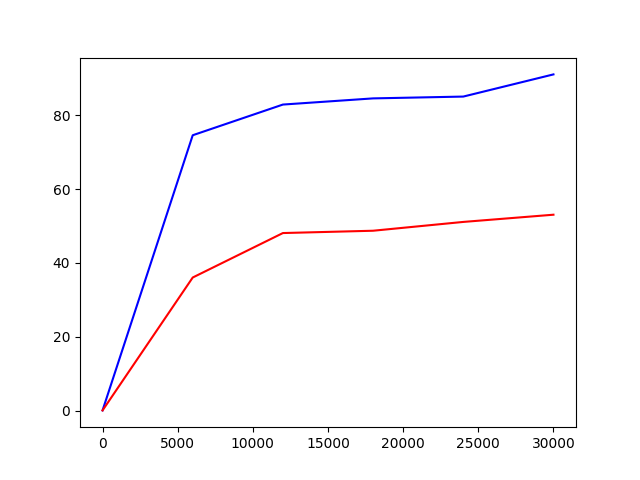
\includegraphics[scale=.5]{learning_curves.png}
		\caption{The learning curves for my (red) and pytorch's (blue) 2 layer neural networks on the MNIST dataset. The $ x $ axis represents the number of samples processed, and $ y $ the percentage accuracy on the validation set.}\label{fig1}
	\end{figure}
	
	
	Next I took the pytorch version (which was much faster and converged better) and changed my weight initializations. For one, I initialized the weights uniformly at random between -1 and 1, and for the other at a constant 0. As I had noticed on my own implementation as well, initializing to 0 makes convergence much slower. The final accuracy for the random initialization was
	\[ 66.4\% \]
	and for the 0 initialization it was
	\[ 68.8\%. \]
	The two learning curves are shown in Figure \ref{fig2}.
	
	\begin{figure}[h]
		\centering
		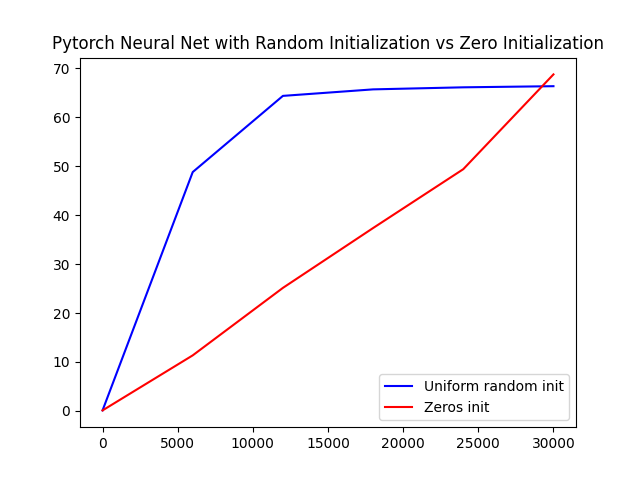
\includegraphics[scale=.5]{inits.png}
		\caption{The learning curves for the different weight initializations.}\label{fig2}
	\end{figure}
	
	\end{enumerate}
	\bibliographystyle{apalike}
\end{document}
